% id: 0275
% book: RPM 중3-2 수학 · 03 원과 직선
% section: 유형 03 현의 수직이등분선 (3)
% figure: crop:fig-0275.png
% answer: $4\mkern3mu \mathrm{cm}$
% answer_source: 답지
% variant_level: 0 (원본 전사)
% 이 파일은 build.mjs 가 items.json 에서 만든다. 고칠 때는 items.json 을 고친다.
\noindent\begin{minipage}[t]{0.58\linewidth}\vspace{0pt}\raggedright 오른쪽 그림에서 $\arc{AB}$는 반지름의 길이가 $20\mkern3mu \mathrm{cm}$인 원의 일부분이다. $\seg{AB}\perp\seg{CD}$, $\seg{AD}=\seg{BD}$이고 $\seg{AB}=24\mkern3mu \mathrm{cm}$일 때, $\seg{CD}$의 길이를 구하시오.\end{minipage}\hfill\begin{minipage}[t]{0.4\linewidth}\vspace{0pt}\centering \setlength{\dmfigw}{95.2pt}\ifdim\dmfigw>\linewidth\setlength{\dmfigw}{\linewidth}\fi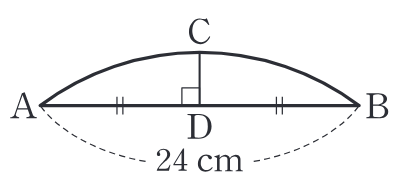
\includegraphics[width=\dmfigw]{figures/fig-0275.png}\end{minipage}\par
